% Part 1 - Document Setup and Preamble
\documentclass[11pt,a4paper]{article}
\usepackage[margin=1in]{geometry}
\usepackage{amsmath}
\usepackage{amssymb}
\usepackage{titlesec}
\usepackage{enumitem}
\usepackage{xcolor}
\usepackage[most]{tcolorbox}
\usepackage{fancyhdr}
\usepackage{listings}
\usepackage{hyperref}
\usepackage{graphicx}
\usepackage{tikz}
\usetikzlibrary{shapes.geometric, arrows, positioning}

% Header and Footer
\pagestyle{fancy}
\fancyhf{}
\rhead{FastAPI Complete Guide}
\lhead{Modern API Development}
\cfoot{\thepage}

% Title formatting
\titleformat{\section}{\Large\bfseries\color{blue!70!black}}{\thesection}{1em}{}[\titlerule]
\titleformat{\subsection}{\large\bfseries\color{blue!50!black}}{\thesubsection}{1em}{}
\titleformat{\subsubsection}{\normalsize\bfseries\color{blue!40!black}}{\thesubsubsection}{1em}{}

% Code styling
\definecolor{codebg}{gray}{0.95}
\definecolor{codegreen}{rgb}{0,0.6,0}
\definecolor{codegray}{rgb}{0.5,0.5,0.5}
\definecolor{codepurple}{rgb}{0.58,0,0.82}

\lstdefinestyle{pythonstyle}{
    language=Python,
    backgroundcolor=\color{codebg},
    commentstyle=\color{codegreen},
    keywordstyle=\color{blue},
    numberstyle=\tiny\color{codegray},
    stringstyle=\color{codepurple},
    basicstyle=\ttfamily\small,
    breaklines=true,
    captionpos=b,
    keepspaces=true,
    numbers=left,
    numbersep=5pt,
    showspaces=false,
    showstringspaces=false,
    showtabs=false,
    tabsize=4,
    frame=single,
    xleftmargin=2em,
    framexleftmargin=1.5em
}

\lstdefinestyle{bashstyle}{
    language=bash,
    backgroundcolor=\color{codebg},
    basicstyle=\ttfamily\small,
    breaklines=true,
    frame=single,
    xleftmargin=2em,
    framexleftmargin=1.5em
}

\lstset{style=pythonstyle}

% Command box
\newtcolorbox{cmdbox}{
    colback=codebg,
    colframe=black!50,
    boxrule=0.5pt,
    left=2mm,
    right=2mm,
    top=1mm,
    bottom=1mm,
    breakable
}

% Example box
\newtcolorbox{examplebox}[1]{
    colback=green!5!white,
    colframe=green!75!black,
    title=#1,
    fonttitle=\bfseries,
    breakable,
    enhanced jigsaw
}

% Note box
\newtcolorbox{notebox}{
    colback=yellow!10!white,
    colframe=orange!75!black,
    title=Important Note,
    fonttitle=\bfseries,
    breakable,
    enhanced jigsaw
}

% Warning box
\newtcolorbox{warningbox}{
    colback=red!5!white,
    colframe=red!75!black,
    title=Warning,
    fonttitle=\bfseries,
    breakable,
    enhanced jigsaw
}

% Info box
\newtcolorbox{infobox}[1]{
    colback=blue!5!white,
    colframe=blue!75!black,
    title=#1,
    fonttitle=\bfseries,
    breakable,
    enhanced jigsaw
}

\begin{document}

% Title Page
\begin{titlepage}
    \centering
    \vspace*{2cm}
    {\Huge\bfseries FastAPI\\[0.5cm] Complete Reference Guide\par}
    \vspace{1cm}
    {\Large Modern API Development with Python\par}
    \vspace{2cm}
    {\large A Comprehensive Guide to Building\\
    High-Performance APIs with FastAPI\par}
    \vspace{3cm}
    {\Large\bfseries Learning Notes\par}
    \vspace{0.5cm}
    {\large Based on Industry Best Practices\par}
    \vspace{3cm}
    {\Large\bfseries Sujil S\par}
    \vspace{0.5cm}
    {\large\texttt{sujil9480@gmail.com}\par}
    \vfill
    {\large \today\par}
\end{titlepage}

\tableofcontents
\newpage

% ========================
% SECTION 1: INTRODUCTION
% ========================
\section{Introduction to FastAPI}

\subsection{What is FastAPI?}

\begin{infobox}{Definition}
\textbf{FastAPI is a modern, high-performance web framework for building APIs with Python.}
\end{infobox}

FastAPI is a Python framework that enables developers to build high-performance, industry-grade APIs efficiently. It captures the essence of modern API development by combining speed, ease of use, and robust features.

\subsection{Why FastAPI for Data Science and AI/ML?}

FastAPI has become essential for professionals working in:

\begin{itemize}[leftmargin=*]
    \item \textbf{Data Science}: Deploy data analysis pipelines as APIs
    \item \textbf{Machine Learning}: Serve ML models in production
    \item \textbf{Artificial Intelligence}: Create AI-powered applications
    \item \textbf{Deep Learning}: Deploy neural networks as web services
\end{itemize}

\begin{notebox}
In modern ML/AI workflows, building an API is often the final step to make your models accessible to applications, allowing them to serve predictions in real-time.
\end{notebox}

\subsection{The Foundation: Built on Two Libraries}

FastAPI is built on top of two popular Python libraries:

\subsubsection{1. Starlette}

\textbf{Starlette} is responsible for handling HTTP communication in FastAPI.

\begin{itemize}[leftmargin=*]
    \item \textbf{Role}: Manages how your API receives requests and sends back responses
    \item \textbf{Functionality}: Handles all HTTP request/response processing
    \item \textbf{Performance}: Provides asynchronous request handling
\end{itemize}

\textbf{What it does}:
\begin{itemize}[leftmargin=*]
    \item Receives HTTP requests from clients
    \item Processes the request data
    \item Sends HTTP responses back to clients
    \item Manages the web server interface
\end{itemize}

\subsubsection{2. Pydantic}

\textbf{Pydantic} is a data validation library used in FastAPI.

\begin{itemize}[leftmargin=*]
    \item \textbf{Role}: Validates incoming data format and types
    \item \textbf{Purpose}: Ensures data integrity and type safety
    \item \textbf{Benefit}: Automatic data validation without manual checks
\end{itemize}

\begin{examplebox}{Why Pydantic is Important in APIs}
Consider an API that takes two station names and a date to return train information:

\textbf{Without Pydantic}: You must manually check:
\begin{itemize}[leftmargin=*]
    \item Are station names in string format?
    \item Are they from the valid list of stations?
    \item Is the date in correct format?
\end{itemize}

\textbf{With Pydantic}: All these checks happen automatically behind the scenes!
\end{examplebox}

\subsection{Architecture Overview}

\begin{center}
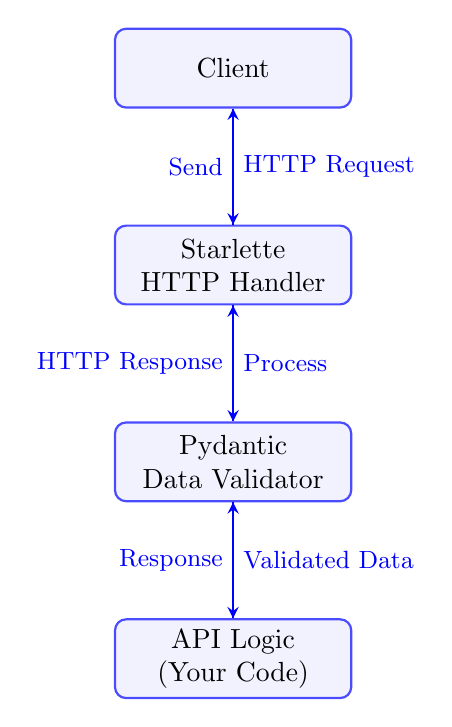
\begin{tikzpicture}[
    node distance=2.5cm,
    box/.style={rectangle, rounded corners, draw=blue!70, fill=blue!5, thick, minimum width=3cm, minimum height=1cm, align=center},
    arrow/.style={->, >=stealth, thick, blue}
]

% Nodes
\node[box] (client) {Client};
\node[box, below of=client] (starlette) {Starlette\\HTTP Handler};
\node[box, below of=starlette] (pydantic) {Pydantic\\Data Validator};
\node[box, below of=pydantic] (api) {API Logic\\(Your Code)};

% Arrows
\draw[arrow] (client) -- node[right, font=\small] {HTTP Request} (starlette);
\draw[arrow] (starlette) -- node[right, font=\small] {Process} (pydantic);
\draw[arrow] (pydantic) -- node[right, font=\small] {Validated Data} (api);
\draw[arrow] (api) -- node[left, font=\small] {Response} (pydantic);
\draw[arrow] (pydantic) -- node[left, font=\small] {HTTP Response} (starlette);
\draw[arrow] (starlette) -- node[left, font=\small] {Send} (client);

\end{tikzpicture}
\end{center}

\newpage

% ========================
% SECTION 2: CORE PHILOSOPHY
% ========================
\section{Core Philosophy of FastAPI}

\subsection{The Two Primary Objectives}

FastAPI was created to solve two major problems that existed with older frameworks like Flask:

\begin{enumerate}[leftmargin=*]
    \item \textbf{Performance Issues}: Older frameworks had slow response times and latency issues
    \item \textbf{Development Complexity}: Writing APIs required extensive boilerplate code
\end{enumerate}

\subsection{Philosophy 1: Fast to Run}

\begin{infobox}{Fast to Run}
FastAPI-built APIs are \textbf{fast in execution}, meaning they:
\begin{itemize}[leftmargin=*]
    \item Handle requests very quickly
    \item Support concurrent users efficiently
    \item Have minimal latency
    \item Perform well under load
\end{itemize}
\end{infobox}

\subsection{Philosophy 2: Fast to Code}

\begin{infobox}{Fast to Code}
FastAPI makes API development \textbf{fast to write}, meaning:
\begin{itemize}[leftmargin=*]
    \item Less boilerplate code required
    \item Fewer lines of code needed
    \item Quick development cycle
    \item Clean, readable syntax
\end{itemize}
\end{infobox}

\begin{notebox}
The name "FastAPI" reflects both philosophies:
\begin{itemize}[leftmargin=*]
    \item \textbf{Fast} = Fast to run (performance)
    \item \textbf{Fast} = Fast to code (development speed)
\end{itemize}
\end{notebox}

\newpage

% ========================
% SECTION 3: HOW APIs WORK
% ========================
\section{Understanding API Architecture}

\subsection{API Components}

Every API consists of two essential components:

\begin{enumerate}[leftmargin=*]
    \item \textbf{API Code}: The business logic that processes requests
    \item \textbf{Web Server}: The component that listens for HTTP requests
\end{enumerate}

\subsection{Complete Request-Response Flow}

Let's understand the complete flow using a machine learning prediction API example:

\begin{examplebox}{Example Scenario}
\textbf{API Endpoint}: \texttt{/predict}

\vspace{0.3em}

\textbf{Inputs}: 
\begin{itemize}[leftmargin=*]
    \item Feature1: some value
    \item Feature2: some value
\end{itemize}

\textbf{Output}: Model prediction
\end{examplebox}

\subsubsection{Step-by-Step Flow}

\hspace{1.6em}\textbf{Step 1: Client Makes Request}
\begin{itemize}[leftmargin=*]
    \item User sends feature values to the API endpoint
    \item Browser/software converts this into an HTTP request
\end{itemize}

\textbf{Step 2: HTTP Request Creation}

\begin{itemize}[leftmargin=*]
    \item Request method (POST, GET, etc.)
    \item Endpoint URL (\texttt{/predict})
    \item Headers (Content-Type, Content-Length, etc.)
    \item Body (Feature values)
    \item Host URL
\end{itemize}

\textbf{Step 3: Web Server Receives Request}
\begin{itemize}[leftmargin=*]
    \item Web server listens on ports continuously
    \item Captures incoming HTTP request
    \item Passes it to the gateway interface
\end{itemize}

\textbf{Step 4: Server Gateway Interface (SGI)}
\begin{itemize}[leftmargin=*]
    \item Acts as a translator between HTTP and Python
    \item Converts HTTP format to Python-understandable format
    \item Enables two-way communication
\end{itemize}

\begin{warningbox}
\textbf{The Problem}: Python cannot directly understand HTTP requests!

\vspace{0.5em}
\textbf{The Solution}: Server Gateway Interface (SGI) translates between HTTP and Python formats.
\end{warningbox}

\textbf{Step 5: API Code Execution}
\begin{itemize}[leftmargin=*]
    \item Python code receives feature values
    \item Loads ML model
    \item Calls prediction function
    \item Generates result
\end{itemize}

\textbf{Step 6: Response Generation}
\begin{itemize}[leftmargin=*]
    \item Python output converted back to HTTP format by SGI
    \item Status code added (e.g., 200 for success)
    \item Response headers added
    \item Complete HTTP response created
\end{itemize}

\vspace{0.2em}
\textbf{Step 7: Response Sent to Client}
\begin{itemize}[leftmargin=*]
    \item Web server sends HTTP response
    \item Client receives prediction result
\end{itemize}

\subsection{Visual Flow Diagram}

\begin{center}
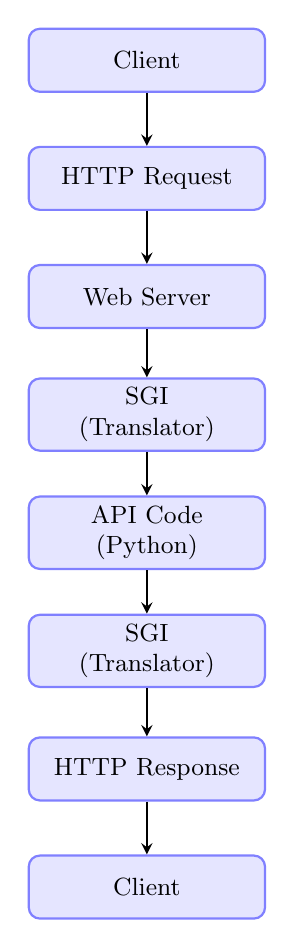
\begin{tikzpicture}[
    node distance=1.5cm,
    process/.style={rectangle, rounded corners, draw=blue!50, fill=blue!10, thick, minimum width=3cm, minimum height=0.8cm, font=\small, align=center},
    arrow/.style={->, >=stealth, thick}
]

% Nodes
\node[process] (client) {Client};
\node[process, below of=client] (http1) {HTTP Request};
\node[process, below of=http1] (webserver) {Web Server};
\node[process, below of=webserver] (sgi) {SGI\\(Translator)};
\node[process, below of=sgi] (apicode) {API Code\\(Python)};
\node[process, below of=apicode] (sgi2) {SGI\\(Translator)};
\node[process, below of=sgi2] (http2) {HTTP Response};
\node[process, below of=http2] (client2) {Client};

% Arrows
\draw[arrow] (client) -- (http1);
\draw[arrow] (http1) -- (webserver);
\draw[arrow] (webserver) -- (sgi);
\draw[arrow] (sgi) -- (apicode);
\draw[arrow] (apicode) -- (sgi2);
\draw[arrow] (sgi2) -- (http2);
\draw[arrow] (http2) -- (client2);

\end{tikzpicture}
\end{center}

\newpage

% ========================
% SECTION 4: FLASK VS FASTAPI
% ========================
\section{Flask vs FastAPI: Architecture Comparison}

\subsection{Flask Architecture}

Flask is a traditional, well-established Python web framework. Let's examine its components:

\subsubsection{Flask Components}

\begin{enumerate}[leftmargin=*]
    \item \textbf{SGI Protocol}: WSGI (Web Server Gateway Interface)
    \item \textbf{WSGI Implementation}: Werkzeug library
    \item \textbf{Web Server}: Gunicorn
    \item \textbf{API Code}: Synchronous Python code
\end{enumerate}

\subsubsection{WSGI (Web Server Gateway Interface)}

\begin{infobox}{What is WSGI?}
WSGI is a specification that standardizes how web servers and Python web applications/frameworks communicate.

\vspace{0.5em}
\textbf{Key Characteristics}:
\begin{itemize}[leftmargin=*]
    \item Older, mature protocol
    \item \textbf{Synchronous} in nature
    \item Processes one request at a time
    \item \textbf{Blocking architecture}
\end{itemize}
\end{infobox}

\begin{warningbox}
\textbf{The Biggest Problem with WSGI}:

WSGI follows a \textbf{synchronous, blocking architecture}.

\vspace{0.5em}
\textbf{What this means}:
\begin{itemize}[leftmargin=*]
    \item Can process only ONE request at a time
    \item When processing one request, others must wait
    \item Resources are blocked during processing
    \item Leads to slower response times
    \item Creates scalability challenges
\end{itemize}
\end{warningbox}

\subsubsection{Example: Multiple Clients}

\begin{examplebox}{WSGI Limitation}
\textbf{Scenario}: 5 clients send requests simultaneously

\vspace{0.5em}

\textbf{What happens}:
\begin{enumerate}[leftmargin=*]
    \item Web server receives all 5 HTTP requests
    \item WSGI starts processing Request 1
    \item Requests 2, 3, 4, 5 wait in queue
    \item Only after Request 1 completes, Request 2 starts
    \item This continues sequentially for all requests
\end{enumerate}

\textbf{Result}: High latency and poor performance under load
\end{examplebox}

\subsubsection{Werkzeug}

\begin{infobox}{Werkzeug Library}
Werkzeug is a comprehensive WSGI web application library.

\vspace{0.5em}
\textbf{Role}: Implements the WSGI protocol for Flask
\end{infobox}

\textbf{Note}: When you install Flask, Werkzeug is automatically installed as a dependency.

\subsubsection{Gunicorn Web Server}

\begin{infobox}{Gunicorn (Green Unicorn)}
Gunicorn is a WSGI HTTP server specifically designed for Python web applications.

\vspace{0.5em}
\textbf{Known for}:
\begin{itemize}[leftmargin=*]
    \item Efficiency in standard use cases
    \item Decent scalability
    \item Wide adoption in Flask applications
\end{itemize}
\end{infobox}

\begin{warningbox}
\textbf{Gunicorn Limitations}:

\vspace{0.5em}

Being WSGI-based, Gunicorn suffers from:
\begin{itemize}[leftmargin=*]
    \item Synchronous processing bottlenecks
    \item I/O wait times
    \item High latency under concurrent load
    \item Performance issues at scale
\end{itemize}
\end{warningbox}

\subsubsection{Flask API Code}

Flask API code is written in standard, synchronous Python:
\begin{itemize}[leftmargin=*]
    \item Processes one request at a time
    \item No built-in concurrency support
    \item Blocking operations halt execution
\end{itemize}

\subsection{Flask Architecture Summary}

\begin{center}
\begin{tabular}{|l|l|}
\hline
\textbf{Component} & \textbf{Flask Choice} \\
\hline
SGI Protocol & WSGI (Synchronous) \\
\hline
WSGI Implementation & Werkzeug \\
\hline
Web Server & Gunicorn \\
\hline
API Code & Synchronous Python \\
\hline
Processing Model & Sequential/Blocking \\
\hline
\end{tabular}
\end{center}

\begin{notebox}
\textbf{Key Takeaway}: Flask's entire pipeline is synchronous, which means:
\begin{itemize}[leftmargin=*]
    \item Only one request processed at a time
    \item Other requests wait in queue
    \item Performance degrades with concurrent users
\end{itemize}
\end{notebox}

\newpage

\subsection{FastAPI Architecture}

FastAPI takes a fundamentally different approach by using asynchronous components throughout the stack.

\subsubsection{FastAPI Components}

\begin{enumerate}[leftmargin=*]
    \item \textbf{SGI Protocol}: ASGI (Asynchronous Server Gateway Interface)
    \item \textbf{ASGI Implementation}: Starlette library
    \item \textbf{Web Server}: Uvicorn
    \item \textbf{API Code}: Async/Await Python code
\end{enumerate}

\subsubsection{ASGI (Asynchronous Server Gateway Interface)}

\begin{infobox}{What is ASGI?}
ASGI is a modern, asynchronous interface for Python web applications.

\vspace{0.5em}
\textbf{Key Characteristics}:
\begin{itemize}[leftmargin=*]
    \item Newer protocol designed for modern needs
    \item \textbf{Asynchronous} in nature
    \item Processes multiple requests concurrently
    \item \textbf{Non-blocking architecture}
\end{itemize}
\end{infobox}

\begin{examplebox}{ASGI vs WSGI}
\textbf{Google Search Result}:

\vspace{0.5em}

``WSGI is an older synchronous interface for Python web applications, while ASGI is a newer asynchronous interface that's better suited for modern web applications like those using WebSockets and real-time features.''
\end{examplebox}

\textbf{The Biggest Advantage of ASGI}:

\begin{itemize}[leftmargin=*]
    \item Can handle \textbf{concurrent requests}
    \item Multiple requests processed in parallel
    \item Non-blocking I/O operations
    \item Superior performance under load
\end{itemize}

\subsubsection{Starlette}

\begin{infobox}{Starlette Library}
``The little ASGI framework that shines.''

\vspace{0.5em}

\textbf{Role}: Implements ASGI protocol for FastAPI

\vspace{0.5em}

\textbf{Capabilities}:
\begin{itemize}[leftmargin=*]
    \item Asynchronous request handling
    \item Concurrent processing support
    \item High-performance HTTP operations
\end{itemize}
\end{infobox}

\subsubsection{Uvicorn Web Server}

\begin{infobox}{Uvicorn}
Uvicorn is a high-performance ASGI server.

\vspace{0.5em}
\textbf{Comparison with Gunicorn}:
\begin{itemize}[leftmargin=*]
    \item Uvicorn: ASGI server (asynchronous)
    \item Gunicorn: WSGI server (synchronous)
\end{itemize}
\end{infobox}

\begin{examplebox}{Performance Comparison}
\textbf{Search Result}: ``Uvicorn vs Gunicorn''

\vspace{0.5em}

``Uvicorn and Gunicorn are both Python web servers, but they cater to different use cases:

\begin{itemize}[leftmargin=*]
    \item \textbf{Uvicorn}: High-performance ASGI server (NOT WSGI)
    \item \textbf{Gunicorn}: Mature WSGI server
\end{itemize}

Uvicorn is generally preferred for its high performance and asynchronous capabilities.''
\end{examplebox}

\subsubsection{Async/Await in Python}

FastAPI supports Python's \texttt{async/await} syntax, enabling true asynchronous processing.

\begin{examplebox}{How Async/Await Works}
\textbf{Scenario}: API endpoint calls ML model for prediction

\vspace{0.5em}
\textbf{Without async/await (Synchronous)}:
\begin{enumerate}[leftmargin=*]
    \item Request arrives at API
    \item API sends input to ML model
    \item \textbf{API waits} while model processes (blocking)
    \item During wait time, \textbf{no other requests can be handled}
    \item Model returns prediction
    \item API sends response
    \item \textbf{Only now} can next request be processed
\end{enumerate}

\textbf{With async/await (Asynchronous)}:
\begin{enumerate}[leftmargin=*]
    \item Request arrives at API
    \item API sends input to ML model with \texttt{await}
    \item \textbf{API continues accepting other requests} while model processes
    \item When model finishes, API sends response
    \item \textbf{Multiple requests processed concurrently}
\end{enumerate}
\end{examplebox}

\begin{lstlisting}[language=Python, caption=Async/Await Example]
# Without async/await (Blocking)
def predict(features):
    result = ml_model.predict(features)  # Blocks here
    return result

# With async/await (Non-blocking)
async def predict(features):
    result = await ml_model.predict(features)  # Doesn't block
    return result
\end{lstlisting}

\subsection{FastAPI Architecture Summary}

\begin{center}
\begin{tabular}{|l|l|}
\hline
\textbf{Component} & \textbf{FastAPI Choice} \\
\hline
SGI Protocol & ASGI (Asynchronous) \\
\hline
ASGI Implementation & Starlette \\
\hline
Web Server & Uvicorn \\
\hline
API Code & Async/Await Python \\
\hline
Processing Model & Concurrent/Non-blocking \\
\hline
\end{tabular}
\end{center}

\subsection{Side-by-Side Comparison}

\begin{center}
\begin{tabular}{|l|l|l|}
\hline
\textbf{Aspect} & \textbf{Flask} & \textbf{FastAPI} \\
\hline
SGI Protocol & WSGI (Sync) & ASGI (Async) \\
\hline
Implementation & Werkzeug & Starlette \\
\hline
Web Server & Gunicorn & Uvicorn \\
\hline
Processing & Sequential & Concurrent \\
\hline
Blocking & Yes & No \\
\hline
Performance & Moderate & High \\
\hline
Scalability & Limited & Excellent \\
\hline
Latency & Higher & Lower \\
\hline
\end{tabular}
\end{center}

\newpage

\subsection{The Restaurant Analogy}

To understand the difference between Flask and FastAPI in simple terms, let's use a restaurant analogy:

\begin{examplebox}{Flask as a Waiter}
\textbf{Flask is like a waiter who}:
\begin{enumerate}[leftmargin=*]
    \item Takes order from Customer 1
    \item Goes to kitchen and gives order to chef
    \item \textbf{Stands in kitchen waiting} while food is being prepared
    \item Takes prepared food back to Customer 1
    \item \textbf{Only then} goes to Customer 2
    \item Repeats the same process
\end{enumerate}

\textbf{Problem}: Time is wasted waiting in the kitchen. Other customers must wait unnecessarily.
\end{examplebox}

\begin{examplebox}{FastAPI as a Waiter}
\textbf{FastAPI is like a waiter who}:
\begin{enumerate}[leftmargin=*]
    \item Takes order from Customer 1
    \item Goes to kitchen and gives order to chef
    \item \textbf{Knows food will take time, so returns to take more orders}
    \item Takes order from Customer 2
    \item Gives it to kitchen
    \item Meanwhile, Customer 1's order is ready
    \item Delivers Customer 1's food
    \item Continues this asynchronous pattern
\end{enumerate}

\textbf{Benefit}: Multiple customers served efficiently. No waiting time wasted.
\end{examplebox}

\begin{notebox}
\textbf{Key Difference}:

\begin{itemize}[leftmargin=*]
    \item \textbf{Flask (Synchronous)}: Waits idle during processing, blocks other requests
    \item \textbf{FastAPI (Asynchronous)}: Serves multiple customers concurrently, maximizes efficiency
\end{itemize}

This is why FastAPI is \textbf{Fast to Run}!
\end{notebox}

\newpage

% ========================
% SECTION 5: FAST TO CODE
% ========================
\section{Why FastAPI is Fast to Code}

\subsection{Three Key Aspects}

FastAPI makes development faster through three main features:

\begin{enumerate}[leftmargin=*]
    \item Automatic Input Validation
    \item Auto-Generated Interactive Documentation
    \item Seamless Modern Library Integration
\end{enumerate}

\subsection{1. Automatic Input Validation}

\subsubsection{The Problem in Python}

Python has dynamic typing by default:
\begin{itemize}[leftmargin=*]
    \item Variables are created dynamically
    \item Types can change at runtime
    \item No built-in type checking
    \item A variable can be integer, then string, etc.
\end{itemize}

\begin{examplebox}{Dynamic Typing Example}
\begin{lstlisting}[language=Python]
# Python allows this:
x = 5           # x is integer
x = "hello"     # now x is string
x = [1, 2, 3]   # now x is list

# No errors - but can cause issues in production!
\end{lstlisting}
\end{examplebox}

\subsubsection{Why This Matters for APIs}

When building enterprise-level APIs, you need to ensure:
\begin{itemize}[leftmargin=*]
    \item Input data is in correct format
    \item Types match expectations
    \item Values are within valid ranges
    \item No type-related runtime errors
\end{itemize}

\subsubsection{FastAPI + Pydantic Solution}

FastAPI integrates tightly with Pydantic for automatic validation:

\begin{lstlisting}[language=Python, caption=Automatic Validation Example]
from fastapi import FastAPI
from pydantic import BaseModel

app = FastAPI()

# Define expected input structure
class PredictionInput(BaseModel):
    feature1: float  # Must be float
    feature2: int    # Must be integer
    feature3: str    # Must be string

@app.post("/predict")
def predict(input_data: PredictionInput):
    # If data doesn't match model, automatic error!
    # No manual checking needed
    return {"prediction": "result"}
\end{lstlisting}

\begin{notebox}
\textbf{Behind the Scenes}:

\vspace{0.5em}
When a request arrives:
\begin{enumerate}[leftmargin=*]
    \item Pydantic automatically checks all types
    \item Validates data format
    \item Converts types if possible
    \item Returns clear error if validation fails
\end{enumerate}

All without writing manual validation code!
\end{notebox}

\subsection{2. Auto-Generated Interactive Documentation}

\subsubsection{The Documentation Challenge}

In traditional API development:
\begin{itemize}[leftmargin=*]
    \item Building the software is one part
    \item Creating documentation is equally important
    \item Users need docs to understand how to use your API
    \item Documentation takes significant time and effort
\end{itemize}

\textbf{For APIs, documentation must include}:
\begin{itemize}[leftmargin=*]
    \item Purpose of each endpoint
    \item Input format expected
    \item Output format returned
    \item Example requests and responses
    \item Error codes and meanings
\end{itemize}

\subsubsection{FastAPI's Solution}

\begin{infobox}{Automatic Documentation}
As you write API code, FastAPI automatically generates:
\begin{itemize}[leftmargin=*]
    \item Complete API documentation
    \item \textbf{Interactive interface} to test endpoints
    \item All endpoint details
    \item Request/response schemas
\end{itemize}
\end{infobox}

\textbf{Accessing Documentation}:

\vspace{0.5em}
Simply navigate to: \texttt{http://your-api-url/docs}

\begin{examplebox}{Interactive Documentation Features}
The auto-generated docs allow you to:
\begin{enumerate}[leftmargin=*]
    \item View all API endpoints
    \item See expected input/output formats
    \item \textbf{Test endpoints directly in browser}
    \item See real-time responses
    \item Understand data models
\end{enumerate}

No need for Postman or other testing tools!
\end{examplebox}

\subsection{3. Seamless Modern Library Integration}

FastAPI is designed with modern development in mind and integrates seamlessly with:

\subsubsection{Machine Learning Libraries}
\begin{itemize}[leftmargin=*]
    \item \textbf{scikit-learn}: Traditional ML models
    \item \textbf{TensorFlow}: Deep learning frameworks
    \item \textbf{PyTorch}: Neural networks
    \item \textbf{XGBoost, LightGBM}: Gradient boosting
\end{itemize}

\subsubsection{Authentication}
\begin{itemize}[leftmargin=*]
    \item \textbf{OAuth}: Social login integration
    \item \textbf{JWT}: Token-based authentication
    \item Built-in security utilities
\end{itemize}

\subsubsection{Database Integration}
\begin{itemize}[leftmargin=*]
    \item \textbf{SQLAlchemy}: SQL databases
    \item \textbf{MongoDB}: NoSQL databases
    \item \textbf{Redis}: Caching solutions
\end{itemize}

\subsubsection{Deployment}
\begin{itemize}[leftmargin=*]
    \item \textbf{Docker}: Containerization
    \item \textbf{Kubernetes}: Orchestration
    \item \textbf{AWS, GCP, Azure}: Cloud platforms
\end{itemize}

\begin{notebox}
\textbf{Why This Matters}:

\vspace{0.5em}
Modern applications require integration with multiple services. FastAPI's tight coupling with these libraries means:
\begin{itemize}[leftmargin=*]
    \item Less boilerplate code
    \item Fewer compatibility issues
    \item Faster development
    \item Better maintainability
\end{itemize}
\end{notebox}

\subsection{Summary: Fast to Code}

\begin{center}
\begin{tabular}{|l|p{0.6\textwidth}|}
\hline
\textbf{Feature} & \textbf{Benefit} \\
\hline
Auto Validation & No manual type checking code \\
\hline
Auto Docs & No separate documentation effort \\
\hline
Modern Integration & Seamless library compatibility \\
\hline
Type Hints & Better IDE support and fewer bugs \\
\hline
Async Support & Write concurrent code easily \\
\hline
\end{tabular}
\end{center}

\newpage

% ========================
% SECTION 6: INSTALLATION & SETUP
% ========================
\section{Installing and Setting Up FastAPI}

\subsection{Prerequisites}

Before installing FastAPI, ensure you have:

\begin{itemize}[leftmargin=*]
    \item \textbf{Python 3.8+}: FastAPI requires Python 3.8 or higher
    \item \textbf{pip}: Python package manager
    \item \textbf{VS Code} (recommended): Or any code editor
    \item \textbf{Terminal/Command Prompt}: For running commands
\end{itemize}

\subsection{Step-by-Step Setup}

\subsubsection{Step 1: Create Project Folder}

\begin{cmdbox}
\begin{verbatim}
# Navigate to desired location (e.g., Desktop)
# Create new folder
mkdir fastapi_tutorials
cd fastapi_tutorials
\end{verbatim}
\end{cmdbox}

\subsubsection{Step 2: Open in VS Code}

\begin{cmdbox}
\begin{verbatim}
# Open VS Code
code .
\end{verbatim}
\end{cmdbox}

Or manually open VS Code and open the folder.

\subsubsection{Step 3: Create Virtual Environment}

\begin{cmdbox}
\begin{verbatim}
# Create virtual environment
python -m venv myenv
\end{verbatim}
\end{cmdbox}

\begin{notebox}
\textbf{Why Virtual Environment?}

\vspace{0.5em}
Virtual environments:
\begin{itemize}[leftmargin=*]
    \item Isolate project dependencies
    \item Prevent version conflicts
    \item Make projects portable
    \item Are Python best practice
\end{itemize}
\end{notebox}

\subsubsection{Step 4: Activate Virtual Environment}

\textbf{On Windows}:
\begin{cmdbox}
\begin{verbatim}
myenv\Scripts\activate.bat
\end{verbatim}
\end{cmdbox}

\textbf{On Linux/Mac}:
\begin{cmdbox}
\begin{verbatim}
source myenv/bin/activate
\end{verbatim}
\end{cmdbox}

You should see \texttt{(myenv)} in your terminal prompt.

\subsubsection{Step 5: Install Required Packages}

\begin{cmdbox}
\begin{verbatim}
# Install FastAPI, Uvicorn, and Pydantic
pip install fastapi uvicorn pydantic
\end{verbatim}
\end{cmdbox}

\textbf{What gets installed}:
\begin{itemize}[leftmargin=*]
    \item \texttt{fastapi}: The FastAPI framework
    \item \texttt{uvicorn}: ASGI web server
    \item \texttt{pydantic}: Data validation library
    \item \texttt{starlette}: Auto-installed with FastAPI
\end{itemize}

Wait for installation to complete. You'll see Starlette being installed automatically as it's a FastAPI dependency.

\subsection{Verifying Installation}

\begin{cmdbox}
\begin{verbatim}
# Check installed packages
pip list

# Look for:
# fastapi
# uvicorn
# pydantic
# starlette
\end{verbatim}
\end{cmdbox}

\newpage

% ========================
% SECTION 7: FIRST API
% ========================
\section{Building Your First FastAPI Application}

\subsection{Hello World API}

Let's build a simple "Hello World" API to understand the basics.

\subsubsection{Step 1: Create Python File}

Create a new file named \texttt{main.py} in your project folder.

\subsubsection{Step 2: Write the Code}

\begin{lstlisting}[language=Python, caption=main.py - Hello World API]
from fastapi import FastAPI

# Create FastAPI app instance
app = FastAPI()

# Define route and endpoint
@app.get("/")
def hello():
    return {"message": "Hello World"}
\end{lstlisting}

\subsection{Code Explanation}

Let's break down each part:

\subsubsection{1. Import FastAPI}

\begin{lstlisting}[language=Python]
from fastapi import FastAPI
\end{lstlisting}

\begin{itemize}[leftmargin=*]
    \item Imports the \texttt{FastAPI} class
    \item This is the main class for creating API applications
\end{itemize}

\subsubsection{2. Create App Instance}

\begin{lstlisting}[language=Python]
app = FastAPI()
\end{lstlisting}

\begin{itemize}[leftmargin=*]
    \item Creates an instance of FastAPI class
    \item This \texttt{app} object is your entire API application
    \item All routes and endpoints are registered with this object
\end{itemize}

\subsubsection{3. Define Route}

\begin{lstlisting}[language=Python]
@app.get("/")
\end{lstlisting}

\vspace{0.5em}
This is a \textbf{decorator} that:
\begin{itemize}[leftmargin=*]
    \item Defines an API route/path
    \item \texttt{get} specifies HTTP GET method
    \item \texttt{"/"} is the URL path (home route)
\end{itemize}

\begin{infobox}{HTTP Methods}
\textbf{GET}: Retrieve/fetch data from server

\vspace{0.5em}
\textbf{POST}: Send/create data on server

\vspace{0.5em}
We use GET here because we're fetching data from the API.
\end{infobox}

\subsubsection{4. Define Handler Function}

\begin{lstlisting}[language=Python]
def hello():
    return {"message": "Hello World"}
\end{lstlisting}

\begin{itemize}[leftmargin=*]
    \item Function executes when route is accessed
    \item Returns a Python dictionary
    \item FastAPI automatically converts to JSON
\end{itemize}

\subsection{Running the API}

\subsubsection{Start the Server}

\begin{cmdbox}
\begin{verbatim}
uvicorn main:app --reload
\end{verbatim}
\end{cmdbox}

\textbf{Command breakdown}:
\begin{itemize}[leftmargin=*]
    \item \texttt{uvicorn}: The ASGI server
    \item \texttt{main}: Python filename (main.py)
    \item \texttt{app}: FastAPI object name
    \item \texttt{--reload}: Auto-reload on code changes
\end{itemize}

\begin{notebox}
\textbf{Why --reload?}

\vspace{0.5em}
The \texttt{--reload} flag:
\begin{itemize}[leftmargin=*]
    \item Watches for code changes
    \item Automatically restarts server
    \item Great for development
    \item Don't use in production!
\end{itemize}
\end{notebox}

\subsubsection{Expected Output}

\begin{cmdbox}
\begin{verbatim}
INFO:     Uvicorn running on http://127.0.0.1:8000
INFO:     Started server process
INFO:     Waiting for application startup.
INFO:     Application startup complete.
\end{verbatim}
\end{cmdbox}

\subsubsection{Test the API}

\textbf{Open your browser and navigate to:}

\begin{center}
\texttt{http://127.0.0.1:8000/}
\end{center}

You should see:
\begin{cmdbox}
\begin{verbatim}
{"message": "Hello World"}
\end{verbatim}
\end{cmdbox}

\subsection{Adding More Endpoints}

Let's add another endpoint to understand multiple routes.

\subsubsection{Updated Code}

\begin{lstlisting}[language=Python, caption=main.py - Multiple Endpoints]
from fastapi import FastAPI

app = FastAPI()

@app.get("/")
def hello():
    return {"message": "Hello World"}

@app.get("/about")
def about():
    return {"message": "CampusX is an education platform where you can learn AI"}
\end{lstlisting}

\subsubsection{What Changed?}

We added a new endpoint:
\begin{itemize}[leftmargin=*]
    \item \textbf{Route}: \texttt{/about}
    \item \textbf{Method}: GET
    \item \textbf{Function}: \texttt{about()}
    \item \textbf{Response}: Information about CampusX
\end{itemize}

\subsubsection{Auto-Reload Magic}

\begin{notebox}
Because we used \texttt{--reload}, the server automatically:
\begin{enumerate}[leftmargin=*]
    \item Detected the code change
    \item Restarted the server
    \item Loaded the new endpoint
\end{enumerate}

No need to manually restart!
\end{notebox}

\subsubsection{Testing Multiple Endpoints}

\hspace{1.2em}\textbf{Test Home Endpoint}:
\begin{center}
\texttt{http://127.0.0.1:8000/}
\end{center}

Response:
\begin{cmdbox}
\begin{verbatim}
{"message": "Hello World"}
\end{verbatim}
\end{cmdbox}

\vspace{0.5em}

\textbf{Test About Endpoint}:
\begin{center}
\texttt{http://127.0.0.1:8000/about}
\end{center}

Response:
\begin{cmdbox}
\begin{verbatim}
{"message": "CampusX is an education platform where you can learn AI"}
\end{verbatim}
\end{cmdbox}

\subsection{Understanding Routes}

\begin{infobox}{How Routes Work}
\textbf{Base URL}: \texttt{http://127.0.0.1:8000}

\vspace{0.5em}
\textbf{Routes}:
\begin{itemize}[leftmargin=*]
    \item \texttt{/} → Home endpoint
    \item \texttt{/about} → About endpoint
    \item Can add any route: \texttt{/users}, \texttt{/products}, etc.
\end{itemize}

Each route connects to a specific function that handles the request.
\end{infobox}

\newpage

% ========================
% SECTION 8: DOCUMENTATION
% ========================
\section{Interactive API Documentation}

\subsection{Accessing Auto-Generated Docs}

FastAPI automatically creates interactive documentation for your API.

\subsubsection{Swagger UI Documentation}

Navigate to:
\begin{center}
\texttt{http://127.0.0.1:8000/docs}
\end{center}

\subsection{What You'll See}

The documentation page displays:

\begin{enumerate}[leftmargin=*]
    \item \textbf{All Endpoints}: List of all API routes
    \item \textbf{HTTP Methods}: GET, POST, etc. for each endpoint
    \item \textbf{Parameters}: Expected inputs for each endpoint
    \item \textbf{Response Models}: Output structure
    \item \textbf{Try It Out}: Interactive testing interface
\end{enumerate}

\subsection{Example Documentation View}

For our current API, you'll see:

\begin{cmdbox}
\begin{verbatim}
GET /
    Returns: {"message": "Hello World"}
    
GET /about
    Returns: {"message": "CampusX is an education..."}
\end{verbatim}
\end{cmdbox}

\subsection{Interactive Testing}

\subsubsection{Step 1: Expand Endpoint}

Click on any endpoint (e.g., \texttt{GET /}) to expand it.

\subsubsection{Step 2: Click "Try it out"}

You'll see a button labeled \textbf{"Try it out"}. Click it.

\subsubsection{Step 3: Execute}

Click the \textbf{"Execute"} button.

\subsubsection{Step 4: View Response}

The documentation will show:

\begin{cmdbox}
\begin{verbatim}
Response Body:
{
  "message": "Hello World"
}

Response Headers:
content-type: application/json
content-length: 26
date: ...
server: uvicorn

Status Code: 200 OK
\end{verbatim}
\end{cmdbox}

\subsection{Benefits of Auto-Documentation}

\begin{enumerate}[leftmargin=*]
    \item \textbf{No Extra Work}: Documentation generated automatically
    \item \textbf{Always Up-to-Date}: Updates with code changes
    \item \textbf{Interactive}: Test endpoints directly
    \item \textbf{Clear Structure}: Well-organized and readable
    \item \textbf{No Postman Needed}: Built-in testing
    \item \textbf{Team Collaboration}: Easy for others to understand your API
\end{enumerate}

\begin{notebox}
\textbf{Amazing Feature}:

As you add more endpoints, parameters, and data models, the documentation automatically updates. You never have to manually write API docs!
\end{notebox}

\subsection{Alternative Documentation}

FastAPI also provides ReDoc documentation:

\vspace{0.5em}
Navigate to:
\begin{center}
\texttt{http://127.0.0.1:8000/redoc}
\end{center}

This provides an alternative, cleaner documentation view.

\newpage

% ========================
% SECTION 9: BASIC CONCEPTS
% ========================
\section{FastAPI Core Concepts}

\subsection{Understanding Decorators}

\subsubsection{What is a Decorator?}

In Python, a decorator is a function that modifies another function's behavior.

\begin{lstlisting}[language=Python, caption=Decorator Syntax]
@app.get("/")  # This is a decorator
def hello():   # This is the function being decorated
    return {"message": "Hello"}
\end{lstlisting}

\subsubsection{What @app.get() Does}

\begin{itemize}[leftmargin=*]
    \item Registers the function as an API endpoint
    \item Associates it with HTTP GET method
    \item Maps it to the specified URL path
    \item Tells FastAPI to execute this function when route is accessed
\end{itemize}

\subsection{HTTP Methods in FastAPI}

\subsubsection{Common HTTP Methods}

\begin{center}
\begin{tabular}{|l|l|p{0.45\textwidth}|}
\hline
\textbf{Method} & \textbf{Decorator} & \textbf{Purpose} \\
\hline
GET & \texttt{@app.get()} & Retrieve/fetch data \\
\hline
POST & \texttt{@app.post()} & Create/send new data \\
\hline
PUT & \texttt{@app.put()} & Update existing data (full) \\
\hline
PATCH & \texttt{@app.patch()} & Update existing data (partial) \\
\hline
DELETE & \texttt{@app.delete()} & Delete data \\
\hline
\end{tabular}
\end{center}

\subsubsection{GET vs POST}

\begin{infobox}{When to Use Each}
\textbf{Use GET when}:
\begin{itemize}[leftmargin=*]
    \item Fetching data from server
    \item Reading information
    \item No data modification
    \item Example: Get user profile, search results
\end{itemize}

\textbf{Use POST when}:
\begin{itemize}[leftmargin=*]
    \item Sending data to server
    \item Creating new resources
    \item Submitting forms
    \item Example: User registration, file upload
\end{itemize}
\end{infobox}

\subsection{Return Values}

\subsubsection{Automatic JSON Conversion}

FastAPI automatically converts Python dictionaries to JSON:

\begin{lstlisting}[language=Python]
@app.get("/")
def hello():
    # You return a Python dict
    return {"message": "Hello", "status": "success"}
    
# FastAPI automatically converts to JSON:
# {"message": "Hello", "status": "success"}
\end{lstlisting}

\subsubsection{What You Can Return}

\begin{itemize}[leftmargin=*]
    \item \textbf{Dictionary}: Converted to JSON object
    \item \textbf{List}: Converted to JSON array
    \item \textbf{Pydantic Models}: Converted to JSON with validation
    \item \textbf{Primitive Types}: strings, numbers, booleans
\end{itemize}

\subsection{Path Parameters}

You can make routes dynamic using path parameters:

\begin{lstlisting}[language=Python, caption=Path Parameters Example]
@app.get("/user/{user_id}")
def get_user(user_id: int):
    return {"user_id": user_id, "name": "John Doe"}

# Access: http://127.0.0.1:8000/user/123
# Response: {"user_id": 123, "name": "John Doe"}
\end{lstlisting}

\subsection{FastAPI Application Object}

\subsubsection{The app Instance}

\begin{lstlisting}[language=Python]
app = FastAPI()
\end{lstlisting}

This \texttt{app} object:
\begin{itemize}[leftmargin=*]
    \item Is your entire API application
    \item Registers all routes and endpoints
    \item Handles request routing
    \item Manages middleware and dependencies
    \item Can be customized with metadata
\end{itemize}

\subsubsection{Customizing the App}

\begin{lstlisting}[language=Python, caption=Custom App Configuration]
app = FastAPI(
    title="My API",
    description="This is my awesome API",
    version="1.0.0"
)
\end{lstlisting}

This information appears in the auto-generated documentation!

\newpage

% ========================
% SECTION 10: PROJECT STRUCTURE
% ========================
\section{Project Organization and Best Practices}

\subsection{Recommended Project Structure}

\begin{cmdbox}
\begin{verbatim}
fastapi_tutorials/
|-- myenv/                 # Virtual environment
|-- main.py                # Main application file
|-- requirements.txt       # Dependencies
|-- .gitignore            # Git ignore file
|-- README.md             # Project documentation
+-- app/                   # Application package (future)
    |-- __init__.py
    |-- models.py          # Data models
    |-- routes.py          # API routes
    +-- config.py          # Configuration
\end{verbatim}
\end{cmdbox}

\subsection{Creating requirements.txt}

To make your project reproducible:

\begin{cmdbox}
\begin{verbatim}
# Generate requirements file
pip freeze > requirements.txt
\end{verbatim}
\end{cmdbox}

This allows others to install dependencies:

\begin{cmdbox}
\begin{verbatim}
# Install from requirements
pip install -r requirements.txt
\end{verbatim}
\end{cmdbox}

\subsection{Development Best Practices}

\begin{enumerate}[leftmargin=*]
    \item \textbf{Use Virtual Environments}: Always isolate project dependencies
    \item \textbf{Use --reload in Development}: Auto-restart on code changes
    \item \textbf{Organize Code}: Separate routes, models, and logic as project grows
    \item \textbf{Write Descriptive Names}: Clear function and route names
    \item \textbf{Use Type Hints}: Helps with auto-completion and validation
    \item \textbf{Test Endpoints}: Use the interactive docs for testing
    \item \textbf{Version Control}: Use Git to track changes
\end{enumerate}

\subsection{Common Commands Reference}

\begin{tcolorbox}[colback=blue!5!white,colframe=blue!75!black,title=Essential Commands]
\begin{verbatim}
# Create virtual environment
python -m venv myenv

# Activate virtual environment
myenv\Scripts\activate.bat          # Windows
source myenv/bin/activate           # Linux/Mac

# Install packages
pip install fastapi uvicorn pydantic

# Run FastAPI server
uvicorn main:app --reload

# Access API
http://127.0.0.1:8000/

# Access documentation
http://127.0.0.1:8000/docs

# Stop server
Ctrl + C
\end{verbatim}
\end{tcolorbox}

\end{document}